\chapter{Architecture and implementation of the Data Integration part}

As stated in the Requirements chapter, the Data Integration part must incrementally pull various REST APIs (data sources) in parallel. For each resource type in
in each data source, it must create an event flow. This event flow run through several data cleaning and data transformation steps that can
be asynchronous. Despite the asynchronous nature, it should ensure that the event flow remains in-order. In the end, event flows are pushed
into the Journal.

\section{Architecture}

\subsection{Puller actor system}

In order to pull periodic incremental pull of data sources, an Akka Actor system is defined. 

First, the system needs for each data source to receive a "top" message corresponding to the fact that a certain data source must be queried. We will use for this
Akka Quartz \footfullcite{bib:akkaquartz}, a cron-style scheduler that allows to define periodic sending of certain types of messages. An usual pull rate for a data source
is every 5 seconds, in order to create a near-realtime stream.
\\

These top messages will be received by a singleton actor named \verb|JobScheduler|. The purpose of the JobScheduler is to launch a child actor for each job (a job
corresponds to an incremental pull from a certain data source). Once the child actor has finished the incremental pull, it kills itself. Figure \ref{fig:archi_actor_dataintegration} illustrates this architecture.

\begin{figure}[h]
  \begin{center} 
    \makebox[\textwidth]{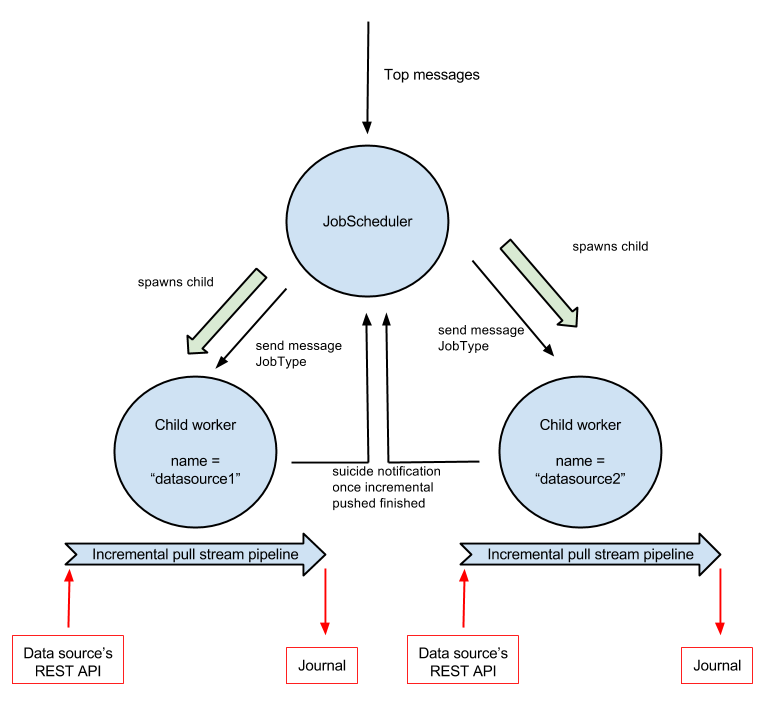
\includegraphics[width=1.0\textwidth]{img/archi_actor_dataintegration.png}}
    \caption{Puller actor system}
    \label{fig:archi_actor_dataintegration}
  \end{center}
\end{figure}

The JobScheduler must handle the fact that the job message rate for a data source can be faster than the incremental pull
of this data source (for example if the data source has produced a lot of new data since the last pull, or if it experiences some network problems). If a pull is still running when 
a new job message arrives for a data source, the JobScheduler should ignore the new pull message to avoid doing two or more pull in parallel of the same data source and risking a wrong
order of events. The JobScheduler can do this by assigning the name of the data source when it spawns a new worker child. Then, when a new job message comes in, it checks if it has a child of this name, and only if such child doesn't exist it spawns a new child.

The actor model also allows to deal with errors. In our case, we just want to ignore the failure of a child worker. The next top message for this data source will automatically
launch a new child worker for this data source. Thus, the JobScheduler actor will have a special Supervision Strategy that ignore the failure of its children.


\subsection{Incremental pull jobs}

When it is launched, each job must do an incremental pull on a particular data source via its REST API. For each the data source that the platform must integrate, there exists
a GET method that allows to get all the resource ids that were updated in a descendant order. The GET response is paginated, meaning that ids are coming 50 by 50 for example (the 
API caller has to make several call until it has all the ids it wants). 

A pull job has to pull the event ids that were updated after the last incremental pull. To do this, we define a stream where the producer makes one or several call to the
paginated REST API to produce a stream of JSON containing the ids of the resources updated. The producer must stop pulling when the date of the current update is less than the last
update event processed during the previous job. In order to persist for each job the date of the last event processed, we use a MongoDB database with a collection that stores a 
document with all the last event processed of each data source.

Moreover, for each resource, we are only interested in keeping the last update. Indeed, the REST API only gives us the type of update with the id of the resource, so if we pull (in desc order) a delete event before an update event, we want only to retain the delete event.

Then, the stream of events should be re-sorted in ascendant order, then for each event we must query the REST API to transform the resource id in the resource itself, then we must clean the resulting JSON to transform it to a known data model, then create an Journal event to insert in the Journal, and finally update MongoDB with the date of the last event.
Figure \ref{fig:datintflow} illustrates this pipeline in a simple schema. 

\begin{figure}[h]
  \begin{center} 
    \makebox[\textwidth]{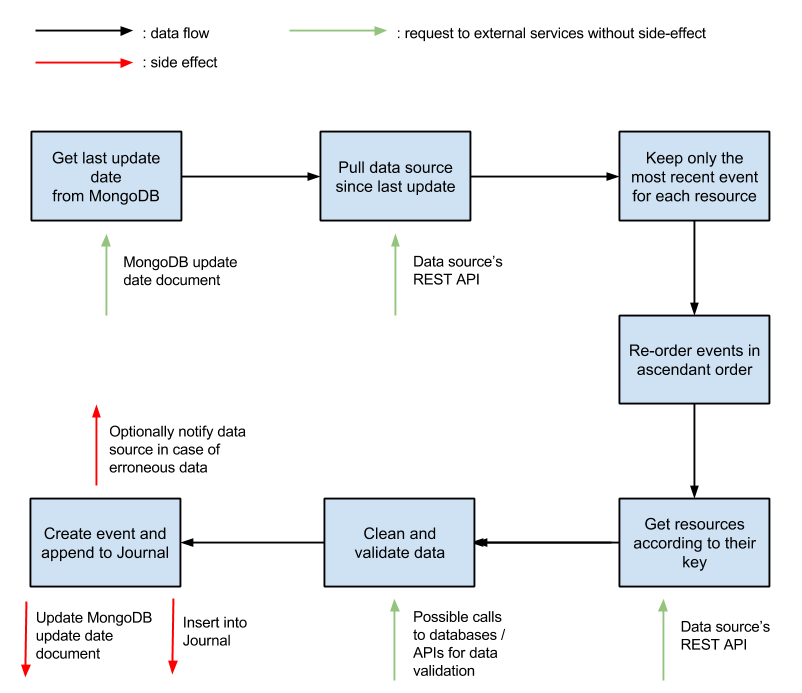
\includegraphics[width=1.0\textwidth]{img/datintflow.png}}
    \caption{Incremental pull stream pipeline}
    \label{fig:datintflow}
  \end{center}
\end{figure}

We see in Figure \ref{fig:datintflow} that the data stream pipeline must asynchronously process (calling external services) events while keeping ordering of messages, so Iteratees and Futures will be used to meet these requirements.
Moreover, an effort is made to isolate side-effects at the end of the stream pipeline in order to enable easy reuse of intermediate blocks. Isolation of side effects for better code
reuse and reasoning is one of the core principles of functional programming.
\\

Such an architecture allows transparent concurrency and parallelism up to the number of cores. Each child actor is executed concurrently, and the asynchronous stream processing
is using Iteratees that use Futures to allow transparent concurrency. If we give to the Iteratees/Futures the SchedulerContext as ExecutionContext, we share threads between actors
and futures, which will create the best possible use of cores in the machine (the total number of threads roughly equals to the number of cores).

Moreover, in case the system needs to scale out, the Actor model also allows easy distribution. In this architecture, the JobScheduler can transparently spawns some worker 
children in other machines. The implementation part will detail this part more thoroughly.


\section{Implementation}

\subsection{Puller actor system}

The Akka framework is used to implement the puller actor system in Scala. The JobScheduler is the main/master actor that receives top messages related to a data source and a special
kind or resource, and spawns a new worker child to accomplish this task only if it has not already a child doing this particular task. Listing \ref{lst:akkajobscheduler} shows the
code of the JobScheduler actor.

\begin{listing}[h]
\begin{minted}[fontsize=\codesize, frame=lines, framesep=2mm]{scala}
class JobScheduler extends Actor {
  private val logger = LazyLogger.apply("services.JobScheduler")

  override val supervisorStrategy = stoppingStrategy
  
  def receive = {
    case jobType: JobMessage =>
      // ensure sequentiality of the iterations of a same job
      val isRunning = context.child(jobType.toString) map (_ => true) getOrElse false
      if (!isRunning) {
        logger.info("Launching child...")
        val worker = context.actorOf(Props[JobWorker], name = jobType.toString)
        worker ! jobType
      } else {
        logger.warn("Job " + jobType + " ignored because the previous iteration 
                                                  of the job is still running.")
      }
  }
}
\end{minted}
\caption{JobScheduler actor}
\label{lst:akkajobscheduler}
\end{listing}

The \verb|supervisorStrategy| is set to \verb|stoppingStrategy| in order to ignore possible failures of children. Listing \ref{lst:akkajobworker} shows the worker actor code.

\begin{listing}[h]
\begin{minted}[fontsize=\codesize, frame=lines, framesep=2mm]{scala}
class JobWorker extends Actor {
  private val logger = LazyLogger.apply("services.JobRunner")
  
  type Job = () => Future[Int]
  case object JobFinished
  
  def receive = {
    case jobType: JobMessage =>
      val job = getLazyJob(jobType)
      job() map { result =>
        logger.info("Finished " + jobType + " job successfully: " + result)
        JobFinished
      } recover { case error: Throwable =>
        logger.error("Finished " + jobType + s" job with error: 
                                  $error\n${error.getStackTraceString}")
        JobFinished
      } pipeTo self
    
    case JobFinished => context.stop(self)
  }

  def getLazyJob: JobMessage => Job = {
    case DataSource1ResourceType1 => DataSource1ResourceType1.job

    case DataSource1ResourceType2 => DataSource1ResourceType2.job

    case DataSource2ResourceType1 => DataSource2ResourceType1.job

    ...
  }
  
}
\end{minted}
\caption{JobWorker actor}
\label{lst:akkajobworker}
\end{listing}

The type \verb|Job| is the type that must be implemented for an incremental pull stream job. \verb|() => Future[_]| means that the pull job must be a function that take no
parameter and return a Future of Int. This Future of Int will be fulfilled when the pull job is finished with the number of Journal events that were created during this iteration
of the incremental pull job. Upon the completion of the future, we map it to a \verb|JobFinished| message that we pipe to \verb|self| (the current actor). Upon the reception
of this message, it knows that the job is finished, and so it kills itself (his parent actor JobScheduler will be automatically notified by its death). Please note that
\verb|context| is part of the actor internal state, so it is not safe to access it into the Future as we saw in section \ref{sec:mixingactorfuture}. That's why we pipe the future to
a message that will be sent to the actor.
\\

The module Akka Quartz allows to define in a configuration file the periodicity of the top messages that will be sent to the JobScheduler actor. See the configuration 
file shown in Listing \ref{lst:configquartz} for an example.

\begin{listing}[h]
\begin{minted}[fontsize=\codesize, frame=lines, framesep=2mm]{scala}
akka {
  quartz {
    schedules {

      DataSource1ResourceType1 {
        description = "Fire DataSource1ResourceType1 every 5 seconds"
        expression  = "*/5 * * ? * *"
      }

      DataSource1ResourceType2 {
        description = "Fire DataSource1ResourceType2 every 2 seconds"
        expression  = "*/2 * * ? * *"
      }

      DataSource2ResourceType1 {
        description = "Fire DataSource2ResourceType1 every 5 seconds"
        expression  = "*/5 * * ? * *"
      }
        
    }
  }
}
\end{minted}
\caption{Cron-style configuration to schedule jobs}
\label{lst:configquartz}
\end{listing}

\subsection{Example of a incremental pull job}

In this section we will describe the implementation of an incremental pull jobs. We take for example a job that pull every 5 seconds the resources of a certain type, called Credit Notes, that has been created, updated or deleted in a SaaS financial software (called FinancialSoftware for this report).
\\

Iteratees and Futures are used to model asynchronous non-blocking stream processing. As we will see, the composabilty of Iteratees allows a very clear modularization of the 
different processing components. 

\subsubsection{Enumerator of Events coming from FinancialSoftware}

The first step is to create an enumerator (a producer) that pull events that happened to a certain resource type since the last pull. The REST API
of FinancialSoftware is paginated by 50, meaning that a GET request on the last events only give the 50 events, and a link the next "page" containing the next 50 events.
The enumerator has to pull the REST API until it detects that the current event has a date inferior to the last update date.
\\

We have to use an enumerator that repeatedly fetch pages from the FinancialSoftware REST API until it has streamed all the events since a date named \verb|since|, and return
a stream of \verb|FinancialSoftwareEvent| containing each the id of a resource of certain type with its related event (create, update or delete) and its date. 
Listing \ref{lst:enumfetchsellsy} shows the code of such enumerator.

\begin{listing}
\begin{minted}[fontsize=\codesize, frame=lines, framesep=2mm]{scala}
case class Page(nb: Int, totalNbPages: Int, docs: Seq[JsObject])
case class FinancialSoftwareEvent(documentId: String, updateType: String, date: DateTime)

object FinancialSoftware {
  private val dateFormat = DateTimeFormat.forPattern("yyyy-MM-dd HH:mm:ss")

  val apiUrl = "..."
  val authentificationParams = "..."

  def retrieveUpdates(resourceType: String, since: DateTime): 
      Enumerator[FinancialSoftwareEvent] = {

    def getPage(nb: Int): Future[Page] = {
      val url = apiUrl + "/" + resourceType + "?" + authentificationParams + "&page=" + nb
      WS.url(url).get map { response =>
        val json = Json.parse(response.body)
        val nbPage = (json \ "pagenum").as[Int]
        val totalNbPages = (json \ "nbpages").as[Int]
        val docs = (json \ "results").as[Seq[JsObject]]
        Page(nbPage, totalNbPages, docs)
      }
    }

    val producer: Enumerator[Seq[JsObject]] = 
      Enumerator.unfoldM[Option[Int], Seq[JsObject]](Some(1)) {
        case Some(nextPageNb) =>
          getPage(nextPageNb) map { nextPage =>
            if (nextPage.nb < nextPage.totalNbPages) {
              Some((Option(nextPage.nb + 1), nextPage.docs))
            } else {
              // last page
              Some(None, nextPage.docs)
            }
          }
        case None => Future.successful(None)
      }

    val flattenedProducer: Enumerator[JsObject] = 
      producer &> Enumeratee.mapConcat(identity)

    flattenedProducer &>
    Enumeratee.map { jsObject =>
      val id = (jsObject \ "relatedid").as[String]
      val date = (jsObject \ "date").as[DateTime]
      val eventType = (jsObject \ "type").as[String]
      FinancialSoftwareEvent(id, eventType, date)
    } &>
    Enumeratee.takeWhile { event =>
      event.date.compareTo(since) > 0
    }
  }
}
\end{minted}
\caption{Enumerator that stream the last events of a data source}
\label{lst:enumfetchsellsy}
\end{listing}

The main method to call is \verb|retrieveUpdates| that returns an Enumerator[FinancialSoftwareEvent]. The \verb|&>| operator between an enumerator and an enumeratee
is an alias for the \verb|through| composition method explained in section \ref{sec:iteratees}.

\subsubsection{Stream pipeline composition}

From this producer of \verb|FinancialSoftwareEvent|, we want to apply several operations to the stream processing pipeline as illustrated in Figure \ref{fig:datintflow}. 
First, we want to keep only the most recent event of each resource. Listing \ref{lst:keepHeadId} shows how to define such an Enumeratee. It returns a 
\verb|Map[String, FinancialSoftwareEvent]| where document id is the key and the last event (so the first in the descendant order stream) related to this document (resource)
is the value.

\begin{listing}[h]
\begin{minted}[fontsize=\codesize, frame=lines, framesep=2mm]{scala}
def groupByDocumentIdKeepingHeadEvent: 
    Enumeratee[FinancialSoftwareEvent, Map[String, FinancialSoftwareEvent]] = {

  Enumeratee.grouped(Iteratee.fold(Map.empty[String, FinancialSoftwareEvent]) { 
    (record, financialEvent) =>
      val id = financialEvent.documentId
      if (!record.contains(id))
        record + (id -> financialEvent)
      else record
  })
}
\end{minted}
\caption{Enumeratee that keeps only the most recent FinancialSoftwareEvent of each resource}
\label{lst:keepHeadId}
\end{listing}

Then, we must create an enumeratee that transform this Map in a stream of event in ascendant date order (see Listing \ref{lst:enumreorder}).

\begin{listing}[h]
\begin{minted}[fontsize=\codesize, frame=lines, framesep=2mm]{scala}
val reorder: Enumeratee[Map[String, FinancialSoftwareEvent], FinancialSoftwareEvent] = 
  Enumeratee.mapConcat { mapIdToEvent => 
    val ascendingSeqOfEvents = mapIdToEvent.toSeq.sortBy { case (id, event) => event.date }
    ascendingSeqOfEvents
  }
\end{minted}
\caption{Enumeratee that re-order events in ascendant order}
\label{lst:enumreorder}
\end{listing}

Then, we must call again the data source's REST API to transform the documentId by the document (resource) itself (see Listing \ref{lst:enumgetdoc}).
Note the use of Enumeratee.mapM that allows sequential (in-order) composition of an asynchronous operation that returns a Future (FinancialSoftware.getResource).

\begin{listing}[h]
\begin{minted}[fontsize=\codesize, frame=lines, framesep=2mm]{scala}
def getDocument(resourceType: String): 
    Enumeratee[FinancialSoftwareEvent, (JsObject, String, DateTime)] =

  Enumeratee.mapM { event =>
    val id = event.documentId
    FinancialSoftware.getResource(resourceType + "/" + id) map { response =>
      (response \ "response").as[JsObject], event.updateType, event.date)
    }
  }
\end{minted}
\caption{Enumeratee that get a resource according to its id}
\label{lst:enumgetdoc}
\end{listing}

Then, several other Enumeratees are created to clean and validate the data that will not be shown here because the code is long and very data specific.
We name this resultant enumeratee cleanAndValidate of type Enumeratee[(JsObject, String, DateTime), Command[ZEvent]], ZEvent being the type of the Journal events. 
Listing \ref{lst:zevent} shows the case class ZEvent which will be more detailed in the Journal and Stream Processing part. 

The \verb|Command| type is a functional type that allows to accumulate the side-effect to do at the end of the pipeline. For example, in the data validation part, the
detection of erroneous data may imply to send a message back to the data source (this type of side-effect is called Annotation). To enhance code re-usability and correctness according to functional programming, the Command type accumulates the different type side-effects that may be done at the end of the pipeline. The final Iteratee that do all the side-effects
is named performSideEffects. It takes a stream of Command[ZEvent], send the possible annotations to the data source, write the possible ZEvent to the Journal and update
the MongoDB collection that stores the date of the last event processed. The type is
Option[ZEvent] because sometimes if data validation fails we don't even want to write an event in the Journal. Listing \ref{lst:finaliterateedataint} illustrates the Command
type and the performSideEffects iteratee (note that for log purpose, the iteratee counts the number of events it has sent to the Journal).

\begin{listing}[h]
\begin{minted}[fontsize=\codesize, frame=lines, framesep=2mm]{scala}
case class ZEvent(
  id: PathId,
  resource: String,
  user: String,
  date: DateTime,
  name: String,
  body: JsObject)
\end{minted}
\caption{ZEvent: a Journal event}
\label{lst:zevent}
\end{listing}

\begin{listing}[h]
\begin{minted}[fontsize=\codesize, frame=lines, framesep=2mm]{scala}
case class Command[A](date: DateTime, maybeEvent: Option[A], annotations: List[Annotation]) 

def performSideEffects: Iteratee[Command[ZEvent], Int] =
  Iteratee.foldM(0) { case (nbEvents, Command(eventDate, maybeEvent, annotations)) =>
    annotations foreach { annotation =>
      annotation.annotate() // send to data source
    }
    maybeEvent match {
      case Some(event) =>
        for {
          _ <- RefJournal.write(event)
          _ <- setLastUpdate(jobKey, eventDate) // set last update date
        } yield nbEvents + 1
      case None =>
        setLastUpdate(jobKey, eventDate) map (_ => nbEvents)
    }
  }
\end{minted}
\caption{PerformSideEffects Iteratee}
\label{lst:finaliterateedataint}
\end{listing}

Thus, we have separately define data producers (enumerator), data transformers (enumeratee) and data sink (iteratee). We now just have to connect them together. Composability
and static typing allows to do so easily, safely and clearly (see Listing \ref{lst:fullpipelinedataint}). The final type of the job method is Job, the alias type for
() => Future[Int] that were defined in the Puller actor system implementation section.

\begin{listing}[h]
\begin{minted}[fontsize=\codesize, frame=lines, framesep=2mm]{scala}
object FinancialSoftware {
  def job: Job = {
    val resourceType = "exampleResource"
    val since = DateTime.now

    val futureLastEventDate = getLastUpdate(resourceType)

    val futureNbEventsInserted: Future[Int] = futureLastEventDate flatMap { lastEventDate =>
      retrieveUpdates("resourceType1", since) &>
      groupByDocumentIdKeepingHeadEvent &>
      reorder &>
      getDocument(resourceType) &>
      cleanAndValidate |>>>  // |>>> is an alias for "run"
      performSideEffects
    }
  }
}

\end{minted}
\caption{Whole stream processing pipeline from a data source to the Journal}
\label{lst:fullpipelinedataint}
\end{listing}


\subsection{Distribution}

This architecture can be easily distributed thanks to actor systems' location transparency. Actually, the above code doesn't need any changes to run it in a distributed
environment. 
For example, we want the worker children that pull DataSource1 to be executed on a remote machine different than the master machine where the JobScheduler actor runs.
We can use the Akka Remote module \footfullcite{bib:akkaremote} for this use case. It allows via a configuration file to configure the JobScheduler actor to create some
of its children in a remote machine rather than locally. The configuration file shown in Listing \ref{lst:configremotemaster} should be put in the master node and 
tells the JobScheduler to create the child actor of names DataSource1ResourceType1 and DataSource1ResourceType2 on the remote machine of address 127.0.0.1:2553.

\begin{listing}[h]
\begin{minted}[fontsize=\codesize, frame=lines, framesep=2mm]{scala}
# Akka master node
akka {
  actor {
    provider = "akka.remote.RemoteActorRefProvider"
    deployment {
      /master/SellsyCreditnotesJob {
        remote = "akka.tcp://remote@127.0.0.1:2553"
      }
    }
  }
  remote {
    enabled-transports = ["akka.remote.netty.tcp"]
    netty.tcp {
      hostname = "127.0.0.1"
      port = 2552
    }
  }
}
\end{minted}
\caption{Configuration file for master node - Akka Remoting}
\label{lst:configremotemaster}
\end{listing}

On the worker machine, an actor system of name "remote" should be launch with the configuration file shown in Listing \ref{lst:configremoteworker}. Moreover,
one should ensure that the JVM classloader on the worker machine has a JAR containing the class JobWorker.

\begin{listing}[h]
\begin{minted}[fontsize=\codesize, frame=lines, framesep=2mm]{scala}
# Akka worker node
akka {
  actor {
    provider = "akka.remote.RemoteActorRefProvider"
  }
  remote {
    enabled-transports = ["akka.remote.netty.tcp"]
    netty.tcp {
      hostname = "127.0.0.1"
      port = 2553
    }
  }
}  
\end{minted}
\caption{Configuration file for worker node - Akka Remoting}
\label{lst:configremoteworker}
\end{listing}

Thus, we transform our system to a mutli-core local system to a distributed system without having to change to code. This can be very useful for systems that first have enough
resources with one machine, but after a while needs to be put on several machines for scalability.
\\

However, one problem with the approach of Akka Remoting is that it is "end-point to end-point" oriented, meaning that the jobs for data source X or Y are statically
mapped to one machine. For elastic and adaptive scalability, it would be more interesting to give a bunch of worker machines to Akka, and it will determine itself on which machine 
it is better to launch the new child worker according to the current resource availability of the machines (CPU, RAM, ...).

This approach in currently under development in Akka and is named Akka Cluster \ref{bib:cluserakka}. In Akka cluster, distribution in cluster centric instead of end-to-end centric, meaning that failed nodes are automatically removed from the cluster, and new node can be added at runtime. Moreover, it will allow automatic actor tree partitioning on the cluster, which means that a given actor child will be automatically created on the machine that is the more available at the current time.

